\section{Задача № 3}

Дано тело \(T\), ограниченное следующими поверхностями:
\( y + \sqrt{x^2 + z^2} = 0, x^2 + z^2 = 1, x^2 + y + z^2 = 2\).

\begin{figure}[!htbp]
  \centering
  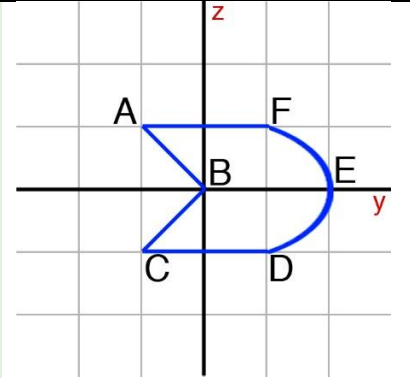
\includegraphics[scale=0.5]{images/Input_task3.png}
\end{figure}

\begin{enumerate}
  \item Изобразите тело \(T\) на графике в пространстве.
  \item Вычислите поток поля
    \[
      \vec{a} = (\sin{zy^2})\vec{i}
      + \sqrt{2} x \vec{j}
      + (\sqrt{2+y}-3z)\Vec{k}
    \]
    через боковую поверхность тела \(T\), образованную вращением дуги \(AFEDC\)
    вокруг оси \(Oy\), в направлении внешней нормали поверхности тела \(T\).
\end{enumerate}

\subsection{Решение}

\begin{figure}[!htbp]
  \centering
  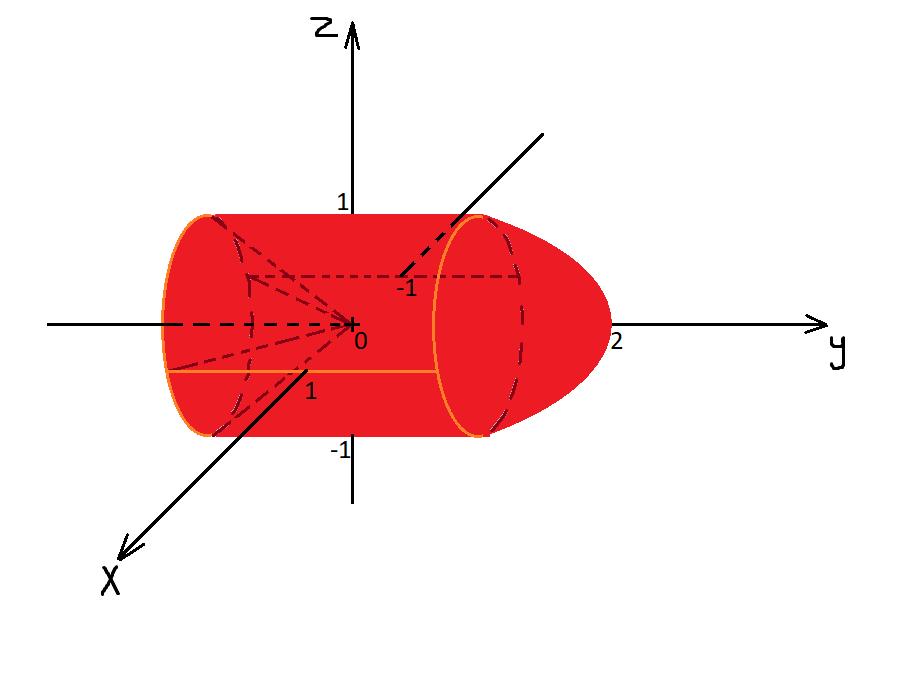
\includegraphics[scale = 0.5]{images/Math_RW4_task3.png}
  \caption{Тело \(T\) в пространстве}
\end{figure}

Поток векторного поля через поверхность ---
это поверхностный интеграл второго рода по поверхности.
\[
  \Pi =
  \iint\limits_{S} P(x,y,z) \dd y \dd z
  + Q(x,y,z) \dd x \dd z
  + R(x,y,z) \dd x \dd y
\]

Векторное поле определено так:
\[
  \vec{a}
  = P(x,y,z)\vec{i} + Q(x,y,z)\vec{j} + R(x,y,z)\vec{k}
  = (\sin{zy^2})\vec{i} + \sqrt{2}x\vec{j} + (\sqrt{2+y}-3z)\vec{k}
\]

Тогда можно получить:
\begin{align*}
  P(x,y,z) &= \sin{z y^2} \\
  Q(x,y,z) &= \sqrt{2}x \\
  R(x,y,z) &= \sqrt{2 + y} - 3z
\end{align*}

Поток векторного поля обладает свойством аддитивности,
поэтому, чтобы найти поток через поверхность,
образованную вращением дуги \(AFEDC\) вокруг оси \(Oy\),
найдем поток через замкнутую поверхность
(\(AFEDC\) замкнутая кривая, вращение вокруг оси \(Oy\)),
затем вычтем поток через поверхность,
образованную вращением отрезка \(AC\) вокруг оси \(Oy\).

\begin{theorem}[Теорема Гаусса-Остроградского]
Поток векторного поля \(\vec{a}\) через
замкнутую кусочно-гладкую поверхность \(S\)
в направлении внешней нормали равен тройному интегралу от
\(\mathrm{div} \vec{a}\) по области \(V\),
ограниченной поверхностью \(S\).
\end{theorem}

Поток через замкнутую поверхность \(\Pi_0\)
найдём по формуле Гаусса-Остроградского:
\[ \Pi_{0} = \iiint_{V} \mathrm{div} \vec{a} \; \dd V \]

Вычислим дивергенцию поля:
\[
  \mathrm{div} \vec{a}
  = \pdv{P(x, y, z)}{x} + \pdv{Q(x, y, z)}{y} + \pdv{R(x, y, z)}{z}
  = 0 + 0 - 3 = -3
\]

Вычисление:
\[
  \Pi_0
  = \iiint_{V} \mathrm{div} \vec{a} \; \dd V
  = \iiint_{V} -3 \dd V
  = -3 \iiint_{V} \dd V
\]

Задача свелась к задаче вычисления объёма фигуры.
Разобъём фигуру на две части: \(-1 \leq y \leq 1\) и \(1 < y \leq 2\).

Первая фигура \(-1 \leq y \leq 1\) --- цилиндр радиусом 1
и высотой \(1 - (-1) = 2\).
Тогда его объём \(V_1 = \pi \cdot 1^2 \cdot 2 = 2 \pi\).

Вторая фигура \(1 < y \leq 2\) задана кривой
\(y = 2 - x^2 - z^2\).
Это эллиптический параболоид, образованный путём вращения
\(y = -\sqrt{x - 2}\) вокруг \(Oy\).
Его объём равен:
\[
  V_2 = \pi \int_{1}^{2} {\left(-\sqrt{-x + 2}\right)}^2 \dd x
  = \pi \int_{1}^{2} (-x + 2) \dd x
  = -\pi \left. \frac{{(-x + 2)}^2}{2}\right\rvert_{1}^{2}
  = -\pi \left(0 - \frac{1}{2}\right)
  = \frac{\pi}{2}
\]

Итого:
\[V = V_1 + V_2 = 2 \pi + \frac{\pi}{2} = \frac{5 \pi}{2}\]

А значит,
\[\Pi_0 = -3 \iiint_{V} \dd V = -3 \frac{5 \pi}{2} = -\frac{15 \pi}{2}\]
Теперь вычислим поток \(\Pi_{1}\) через поверхность,
образованную вращением отрезка \(AC\) вокруг оси \(Oy\).

\[
    \Pi_{1} = \iint_{S} (\vec{a}, \vec{n_{0}}) \dd \sigma
\]
\(\vec{n_0}\) --- это единичный вектор нормали.

Так как образованная поверхность параллельна плоскости \(Oxz\)
и в замкнутой поверхности поток проходил в направлении внешней нормали:
\(\Vec{n_{0}} = \{0,-1,0\}\)

\[(\vec{a}, \vec{n_{0}}) = 0 - \sqrt{2}x + 0 = -\sqrt{2}x\]

Поверхность: \(x^2 + z^2 = 1\)

Вычисление:
\[
\begin{split}
  \Pi_{1} = \iint_{S} -\sqrt{2}x \dd \sigma
    = \iint_{S_{Oxz}} -\sqrt{2}x
      \sqrt{1 + y_{x}^\prime + y_{z}^\prime} \dd x \dd z \\
    = \iint_{S_{Oxz}} -\sqrt{2}x \sqrt{1 + 0 + 0} \dd x \dd z
    = \iint_{S_{Oxz}} -\sqrt{2}x \dd x \dd z
\end{split}
\]

Так как \(S_{Oxz}\) представляет из себя окружность, то перейдём
в ПСК, не забыв про \(J = \rho\) и \(x = \rho \sin\varphi\).
\[
\begin{split}
  \Pi_1
  = \iint_{S_{Oxz}} -\sqrt{2}x \dd x \dd z
  = \int_{0}^{2\varphi} \dd \varphi
    \int_{0}^{1} -\sqrt{2} \rho \sin\varphi \cdot \rho \dd \rho
  = -\sqrt{2} \int_{0}^{2\varphi} \dd \varphi
     \int_{0}^{1} \rho^2 \sin\varphi \dd \rho \\
  = -\sqrt{2} \int_{0}^{2 \varphi} \sin\varphi \dd \varphi
    \int_{0}^{1} \rho^2 \dd \rho
  = -\sqrt{2} \cdot 0 \cdot \int_{0}^{1} \rho^2 \dd \rho
  = 0
\end{split}
\]

Итак, поток поля через боковую поверхность,
образованную вращением дуги \(AFEDC\) вокруг оси \(Oy\) равен:
\begin{equation*}
    \Pi = \Pi_{0} - \Pi_{1} = -\frac{15\pi}{2} - 0 = -\frac{15\pi}{2}
\end{equation*}
